\documentclass{article}
\usepackage[utf8]{inputenc}
\usepackage{graphicx}
\graphicspath{ {images/} }
\usepackage{blindtext}
\begin{document}
\begin{titlepage}
{
\includegraphics[width=0.2\textwidth]{udea.png}\par}
\vspace{1cm}
\centering
{\bfseries\LARGE Universidad de antioquia \par}
\vspace{1cm}
{\scshape\Large Facultad de Ingenieria \par}
\vspace{3cm}
{\scshape\Huge Nociones de la memoria del computador \par}
\vspace{3cm}
\vfill
{\Large Autor: \par}
{\Large arnel david bravo tobon  \par}
\vfill
{\Large septiembre 2020 \par}
\end{titlepage}

\section*{Resumen}
En este documento se hablará de los tipos de memorias que podemos encontrar en un computador, podremos ver que hay memorias temporales donde estas tienen gran importancia para que los procesos se realicen de una manera más eficiente , de solo lectura donde se encuentran las instrucciones de la máquina y se compone por la BIOS y el setup que son esenciales para el funcionamiento del computador y las memorias para almacenar datos que son tan importantes en nuestra vida cotidiana. 

\section*{Introduccion}
La memoria es muy importante ya que Se utiliza para almacenar datos e instrucciones y es muy necesaria para el correcto funcionamiento de la máquina, existen diferentes tipos de memorias en un computador y cada una cumple con una función algunas almacenan información, como otras que solo son temporales o de lectura.


\section*{Funcionamiento de la memoria de un computador}

Si uno se pone a pensar en todos los tipos de memoria electrónica que existen, se encontraría
con un gran número de ellos, muchos de los cuales se han vuelto ya parte de nuestra vida
cotidiana. Algunos de los términos más utilizados para referirse a tipos de memoria electrónica
son:
\begin{itemize}
\item Memoria RAM (Random Access Memory - Memoria de Acceso Aleatorio).
\item Memoria ROM (Read Only Memory - Memoria de sólo lectura).
\item Memoria Cache.
\item Memoria RAM Dinámica o DRAM (Dynamic RAM).
\item Memoria RAM Estática o SRAM (Static RAM).
\item Memoria Flash.
\item Memoria Virtua.
\item Memoria de Video o VRAM
\end{itemize}
Si uno se pone a pensar en todos los tipos de memoria electrónica que existen, se encontraría
con un gran número de ellos, muchos de los cuales se han vuelto ya parte de nuestra vida
cotidiana. Algunos de los términos más utilizados para referirse a tipos de memoria electrónica
son:
\begin{itemize}
\item Teléfonos celulares.
\item Consolas de juego.
\item Reproductoras y grabadoras de DVD.
\item Televisores.
\item Tablets.
\end{itemize}
En este artículo se explican nociones acerca de las memorias de un computador, desde qué
significan los términos más utilizados hasta cómo funcionan.
\section*{La memoria del computador}
La memoria cumple un papel muy importante en el computador y su funcionamiento, ya que se
trata del dispositivo donde se almacena temporalmente toda la información con la que trabajan
los microprocesadores para procesarla y devolver los resultados que los usuarios requieren.\\[0.1cm]
Se podría realizar la siguiente analogía; imaginen un empleado que debe realizar una serie de
tareas contables. El cajón donde se guardan los documentos administrativos, podría
considerarse equivalente a un disco duro; los documentos son equivalentes a los datos e
información a procesar; el escritorio o mesa de trabajo donde se apilan dichos documentos
sería equivalente a la memoria del computador donde se almacena temporalmente la
información que se encuentra en procesamiento; mientras que la persona o su cerebro vendría
a ser como un procesador que realizará las distintas tareas:
\begin{itemize}
\item Primero se sacan del cajón (disco duro) los documentos administrativos y se los lleva a un
escritorio (memoria) donde se apilan para poder trabajar.
\item Se toma un primer documento de la pila para que el empleado (microprocesador) realice
los cálculos necesarios, así como otras tareas y finalmente se ingresan las modificaciones o
resultados de datos procesados en dicho documento.
\item Se regresa dicho documento procesado a otra parte del escritorio (memoria) donde se
colocarán los documentos procesados.
\item Luego se toma otro documento de la pila de documentos no procesados y se repiten los dos
pasos anteriores. Eso se reitera una y otra vez hasta que todos los documentos hayan sido
procesados.
\item Finalmente cuando se terminan de procesar todos los documentos, los cuales se encuentran
apilados en la parte del escritorio (memoria) de documentos ya procesados, se toman y se
vuelven a guardar en el cajón (disco duro) de almacenamiento de archivos.
\end{itemize}
La analogía anterior es una buena comparación del modo de funcionar de un computador; y
específicamente de la memoria. Ahora veamos un ejemplo concreto de cómo funciona la
memoria de un computador en la práctica, durante la realización de una tarea cotidiana.
\begin{itemize}
\item Un usuario se dispone a modificar un documento con un procesador de texto. Para eso abre
un programa de procesamiento de texto que supongamos se llama Word (muy original lo
mio), y que se encuentra almacenado en su disco duro. La orden que le envía este usuario
al computador para abrir dicha aplicación mediante un mouse, viaja en forma de pulsos
eléctricos y llega hasta la memoria, colocándose temporalmente en un espacio de la misma.
Después el microprocesador recibe un aviso de que en una cierta ubicación de la memoria
hay una nueva orden y la pasa a buscar. La misma es leída por el microprocesador,
indicándole que debe abrir un programa de procesamiento de texto llamado Word y que se
encuentra almacenado en el disco duro del computador.
\item A continuación la orden se elimina tanto del procesador como de la memoria, para que
dicho espacio no sea ocupado por algo que ya ha sido utilizado. De esta manera el
procesador le envía la orden a un controlador especial ubicado en la placa madre
(motherboard), que vendría a ser como un empleado de transportes que lleva la
información de un dispositivo a otro. Dicho controlador toma la aplicación llamada Word,
que está almacenada en el disco duro y la lleva hasta la memoria, colocándola en un espacio
vacío de la misma para poder trabajar con ella.
\item El microprocesador comienza a poner en operación a Word una vez ubicado en la memoria.
El microprocesador del computador necesita utilizar la memoria ya que no tiene suficiente
espacio de almacenamiento para trabajar con tanta información, por lo que la almacena
temporalmente en la memoria donde sí hay mucho espacio para poder operar con
información de gran tamaño. Procesa de a partes cada pedazo de la información ubicada en
la memoria, trayéndolos y llevándolos una y otra vez del procesador a la memoria y vice
versa. Una buena analogía es verlo como que un empleado administrativo no tiene
suficiente capacidad de almacenamiento en sus manos para trabajar (procesar) todos los
documentos; por lo que los apoya en su mesa de trabajo o escritorio (memoria) donde hay
más espacio; tomando a cada instante determinado únicamente los documentos que
necesita y luego devolviéndolos a un espacio del escritorio donde puedan ser apoyados
mientras realiza otras tareas.
\item Una vez que Word se encuentra cargado (así se dice técnicamente) en memoria y
funcionando, el usuario envía otra orden con el mouse que le indica al computador que abra
un archivo de texto (supongamos que se llama examen.doc), el cual también se encuentra
almacenado en el disco duro. De esta manera la orden de abrir dicho documento de texto se
carga en un espacio (dirección se dice técnicamente) vacío de memoria donde puede ser
recogido por el microprocesador.
\item El microprocesador luego recibe un aviso de que hay una instrucción aguardando en una
dirección de la memoria. Por lo que la busca, se la lleva y la procesa. La misma como ya
sabemos, le indica que debe abrir un archivo de texto llamado examen.doc que se encuentra
almacenado en el disco duro del computador.
\item A continuación nuestro microprocesador elimina la instrucción ubicada en la memoria para
que no ocupe espacio innecesariamente. Después le envía la orden a ese controlador de
memoria ubicado en la placa madre o motherboard, para que vaya a buscar
a examen.doc del disco duro y lo coloque en la memoria.
\item Dicho controlador toma el archivo del disco duro y lo transporta hasta la memoria
colocándolo en espacios o direcciones vacías de la memoria. Es bueno en este punto explicar
que la información, instrucciones y datos viajan de un dispositivo a otro (microprocesador,
memoria, disco duro, etc) a través de algo llamado bus de datos, que no son otra cosa más
que esas líneas o circuitos impresos de cobre que se ven sobre la placa madre o
motherboard si se abre el computador.
\item Una vez que el archivo examen.doc se encuentra en la memoria; el microprocesador utiliza
los recursos del programa Word que también se encuentra en la memoria, para poder
procesar a examen.doc.
\item Ya en este momento nuestro usuario puede realizar una serie de tareas utilizando las
herramientas del programa Word, con lo que se harán modificaciones en el documento de
texto abierto. Durante esta instancia de trabajo se darán una infinidad de instrucciones,
procesamientos de datos en el microprocesador así como millones de transferencias de
porciones de datos entre la memoria y el microprocesador, las cuales se irán traduciendo a
texto modificado acorde a las necesidades del usuario.
\item Una vez finalizados los trabajos del usuario con el documento, guardará los cambios. En ese
momento el usuario a través del mouse envía la orden de guardar los cambios. Dicha
instrucción viaja hasta la memoria; a continuación el microprocesador recibe un aviso de
nueva orden; la toma de la memoria, la lee y luego la elimina para que no ocupe espacio
innecesario de la memoria.
\item Acto seguido le envía una orden a controlador de memoria, que se encarga de transportar
información de la memoria a otros dispositivos y vice versa a través del bus de datos. Dicha
orden consiste en guardar el documento de texto con el que se trabajó, realizando un copia
exacta en el disco duro de cómo se encuentra modificado y se ve en memoria; también con
su mismo nombre original, examen.doc; lo cual significa que será sobrescrito.
\item Una vez concluidas las tareas, el usuario envía con su mouse la orden de cerrar Word; la
cual viaja a través del cable del mouse hasta la placa madre y una vez ahí a través del bus
de datos hasta la memoria del computador.
\item El microprocesador recibe un aviso de orden, la pasa a buscar de su ubicación en memoria,
la lee y luego la elimina para que no ocupe espacio innecesario de la memoria. Dicha
instrucción le ordena que cierre a Word, lo cual técnicamente no es otra cosa más que
quitarlo del espacio que ocupa en memoria. Por lo tanto procede a quitarlo de la memoria,
así como a examen.doc. ATENCION: No lo elimina del disco duro, que es donde se
encuentra almacenado el original de Word, sino que quita la copia temporal de dicho
programa que se encuentra almacenada temporalmente en la memoria para
trabajar.
\end{itemize}
Lo que se describió recién es lo que ocurre en todo momento cuando trabajamos con un
computador y sintetiza bastante bien la importancia que tiene la memoria para que un sistema
funcione correctamente y pueda realizar todas las tareas.\\[0.1cm]
Aunque técnicamente se considera memoria a todo tipo de dispositivo de almacenamiento
electrónico, usualmente se utiliza el término para referirse a dispositivos de almacenamiento
temporal y alta velocidad de acceso, como lo es la memoria principal del computador.\\[0.1cm]
Pero muchos se preguntarán; por qué en lugar de utilizar la memoria para trabajar, el
microprocesador no utiliza los discos duros; el motivo es simple, velocidad; ya que los discos
duros son mucho más lentos que la memoria, puesto que para acceder a la información se
depende de la velocidad de rotación de los discos que tiene adentro y que son mucho más lentos
que un módulo de memoria que permite acceder a la información almacenada temporalmenteen él en lapsos de tiempo de nanosegundos (mil millonésimas de segundo).\\[0.1cm]
Si el microprocesador tendría que trabajar con el disco duro, todo funcionaría más lentamente,
por lo que se requieren dispositivos más rápidos.\\[0.1cm]
Cuando se está utilizando el computador todas las instrucciones y datos van a parar a la
memoria RAM (Random Access Memory - Memoria de Acceso Aleatorio).\\[0.1cm]
Pero existe un tipo de memoria aún más veloz que la RAM, se trata de la memoria Cache, la cual
es un tipo de memoria más costosa pero mucho más rápida y que se encuentra en todos los
computadores pero que tiene menor capacidad de almacenamiento, dados sus altos costos.
Pueden llegar a tener capacidades de aproximadamente 12 MB (Megabytes) a comparación de
la memoria RAM que cuenta con varios Gigabytes de capacidad.\\[0.1cm]
La memoria Cache se utiliza para trabajar con los datos e instrucciones que el microprocesador
ve que se utilizan más seguido, entonces para no tener que ir a buscarlos una y otra vez de la
memoria RAM que es más lenta, coloca una copia de esos datos en la memoria Cache para
tenerlos a mano. La memoria Cache se encuentra dentro del microprocesador y se divide en
tres niveles (levels en inglés) L1, L2 y L3. La memoria Cache L1 es la más rápida y se encuentra
dentro de los núcleos del microprocesador, la L2 es un poco más lenta pero igualmente hoy día
se encuentra incorporada también dentro del microprocesador (antiguamente se encontraba
al lado del microprocesador en la placa madre) y tiene mayor capacidad que la L1; finalmente
la L3 es la más lenta de las tres pero la que mayor capacidad tiene, siendo aun así mucho más
veloz que la memoria RAM instalada en la placa madre o motherboard del computador.\\[0.1cm]
Por ejemplo en los procesadores de tipo Intel i5 cuentan con memorias Cache L1 dentro de cada
núcleo del procesador las cuales se encuentran divididas en memoria Cache L1 para datos
y memoria Cache L1 para instrucciones de 32 kilobytes cada una. En cuanto a la
memoria Cache L2 de estos procesadores, cada núcleo cuenta con 256 kilobytes para almacenar
tanto datos como instrucciones. Finalmente la memoria Cache L3 se encuentra dentro del
conjunto del procesador pero fuera de los núcleos y es compartida por cada uno de ellos; es
más lenta que las L1 y L2 pero igualmente mucho más rápida que la memoria RAM ubicada en
la placa madre o motherboard; este tipo de modelo de microprocesador cuenta con
aproximadamente 12 Megabytes de L3.\\[0.1cm]
Así en un computador del año 2012 se podía encontrar un microprocesador multinúcleo de 4
núcleos; 32 kilobytes de L1 para datos y 32 kilobytes de L1 para instrucciones en cada núcleo,
dando un total de 256 kilobytes de L1; 256 kilobytes de L2 en cada núcleo para dar un total de
1 Megabyte de L2; y 12 MB de L3 compartidos por todos los núcleos. En cuanto a su memoria
RAM ubicada en la placa madre podía contar con 4 Gigabytes o mucho más de la misma.\\[0.1cm]
Todos los dispositivos del computador; como el microprocesador, el disco duro y la memoria
entre otros, trabajan en equipo, y la memoria podría decirse que es uno de los componentes
más importantes de este equipo. Desde el primer momento en que se enciende el computador
hasta el momento en que se apaga, el microprocesador hace uso constante de la memoria.\\[0.1cm]
Veamos lo que sucede desde que se enciende la máquina:
\begin{itemize}
\item Se enciende el computador y el microprocesador necesita programas o aplicaciones para
funcionar y hacer las distintas tareas, pero como todavía no puede leer nada desde su disco
duro simplemente porque no sabe que existe y tampoco sabe cómo hacerlo; lee las primeras
instrucciones desde un tipo de memoria no volátil (o sea que no se borra) que se encuentra
de fábrica en la placa madre, llamada ROM (Read Only Memory - Memoria de Sólo Lectura);
de ella lee la primera instrucción que se llama POST (Power-On Self-Test - Auto Prueba de
Encendido) la cual le ordena que haga un chequeo de funcionamiento de los componentes
más importantes del sistema. Como parte de esta prueba el controlador de memoria hace
un chequeo de todas las direcciones de memoria para ver que no hayan daños físicos en sus
chips, escribiendo un bit en cada celda de memoria y luego leyendo a cada uno de esos bits
(un bit es un pulso eléctrico, la menor cantidad de información posible en un computador.
\item Una vez que la memoria se encuentra en funcionamiento se carga en la misma un programa
llamado BIOS (Basic Input Output System) que provee información acerca de los
dispositivos de almacenamiento con que cuenta el computador (discos duros, lectoras de
DVD); información sobre cuál es el disco de arranque que contiene el sistema operativo que
se cargará en memoria para poder trabajar con el computador; información sobre
dispositivos como adaptadores de video, sonido y otros con que cuenta el sistema, y otro
tipo de información. Es como una presentación de todos los componentes que forman parte
del equipo; de esta forma cada vez que el microprocesador quiera enviar o recibir una
instrucción de cada uno de éstos, sabrá dónde encontrarlos simplemente buscando su
dirección o identificador cargado en la memoria RAM en el momento en que se encendió la
máquina.
\item Como el microprocesador ya sabe de la existencia del disco duro de arranque, que contiene
un sistema operativo para que podamos trabajar; pasa a cargar dicho sistema operativo en
la memoria RAM (por ejemplo Windows, Linux, Unix o Mac OS, entre otros). El sistema
operativo es lo que permite que podamos manejar el computador e interactuar con ella. Se
puede decir que es el programa más importante de todos y el que permite que podamos
cargar otros programas como juegos, reproductores de audio y video, procesadores de
texto, exploradores Web, etc. El sistema operativo permanece cargado todo el tiempo en la
memoria RAM hasta que se apaga el computador, ya que nuestro microprocesador hará uso
del mismo a cada instante, por lo que lo necesita en la memoria para tener acceso inmediato
a sus recursos.
\item Una vez que se cargó el sistema operativo podemos comenzar a trabajar con el computador.
Cuando se abre un programa o aplicación, el mismo es cargado en la memoria RAM; pero
para conservar espacio de la misma, inicialmente solamente carga las partes esenciales de
dicho programa y eventualmente cargará otros pedazos según sea necesario.
\item Una vez que una aplicación haya sido cargada en la memoria, todo archivo que se abra para
ser utilizado en dicha aplicación también será cargado en la memoria.
\item Una vez que se haya terminado de trabajar con un archivo, si se guardan los cambios
realizados, éstos serán almacenados en el disco duro. Pero cuando se cierra el archivo el
mismo será inmediatamente eliminado o quitado de la memoria RAM, para que dicho
espacio esté disponible a otros recursos.
\item Si se cierra la aplicación con la que trabajamos también se elimina de la memoria.
\end{itemize}
Cada vez que algún archivo o aplicación se abre se carga en la memoria RAM; para que el
microprocesador tenga acceso inmediato a esta información, dado que la memoria es
muchísimas veces más rápida que el disco duro, haciendo que se pueda trabajar más
velozmente.\\[0.1cm]
El microprocesador toma los datos e instrucciones de la memoria RAM, los procesa y devuelve
los resultados ya procesados escribiéndolos en la memoria en un ciclo continuo. Esta ida y
vuelta de datos entre el microprocesador y la memoria ocurre millones de veces por segundo.
Una vez que se cierra una aplicación, ella y los archivos que funcionan bajo la misma (por
ejemplo un editor de imágenes y las imágenes editadas) se quitan instantáneamente de la
memoria, para dar espacio a otros datos. Si los archivos con los que se trabajó no se guardan en
un dispositivo de almacenamiento permanente (como por ejemplo un disco duro) se pierden
para siempre.
\section*{Tipos de memoria de un computador}
En un computador hay varios tipos de memoria, ordenados en jerarquías de velocidad y
capacidad.
\begin{itemize}
\item Memoria Cache L1, L2 y L3
\item Memoria RAM
\item Memoria Virtual
\item Disco Duro
\end{itemize}
Cuanto más bajamos en la lista desde la memoria Cache hacia el disco duro, decrece la velocidad
de los distintos tipos de memoria y aumenta su capacidad.\\[0.1cm]
Los microprocesadores actuales son muy rápidos y funcionan a miles de millones de ciclos por
segundo Ghz (Gigahertz), lo cual significa que pueden procesar miles de millones de bytes por
segundo. Por esta razón requieren de dispositivos de almacenamiento temporal de alta
velocidad que puedan seguirle el ritmo, de lo contrario se detendría para aguardar que la
información le llegue.\\[0.1cm]
Sin embargo hay un pequeño problema, y es que la memoria que puede funcionar a la misma
velocidad del microprocesador es muy cara; y en grandes cantidades harían inalcanzable los
costos de un computador personal hogareña.\\[0.1cm]
Pero los ingenieros encontraron una solución a este problema, utilizando el tipo de memoria
más veloz, Cache, en pequeñas cantidades, y la memoria RAM en mayores cantidades. Cada vez
que el microprocesador se da cuenta que un segmento de datos o información se utiliza de
manera reiterada, toma una copia de la RAM y la carga en la memoria Cache. Y a su vez de esta
información la más utilizada la lleva a la Cache de nivel 1, o sea L1, que se encuentra dentro de
los mismos núcleos del microprocesador, funcionando a la misma velocidad de éstos. Los datos
que utiliza un poco menos los coloca en la memoria Cache L2, que también se encuentra dentro
de los núcleos, pero es un poco más lenta que la anterior, sin embargo puede tener mayor
capacidad, mientras que el resto de la información "cacheada" la coloca en la L3 que puede
llegar a tener como 12 Megabytes en promedio.\\[0.1cm]
En el próximo nivel de jerarquía se encuentra la memoria principal del computador, la memoria
RAM, que a pesar de ser más lenta que la memoria Cache, es muchísimo más rápida que el disco
duro y se puede tener en grandes cantidades a un precio accesible; por lo que cuando se trabaja,
la mayor parte de la información se carga en ella y solamente aquellas pequeñas porciones que
se utilizan seguido van hacia la memoria Cache. De este tipo de memoria hablaremos más
adelante con mucho detalle ya que es la que más nos interesa en este artículo.\\[0.1cm]
Después en el nivel de jerarquías le sigue la memoria virtual que no es otra cosa más que una
porción del disco duro dedicada exclusivamente a "sostener" temporalmente los pedazos de los
programas y datos en ejecución que se utilizan menos o que ocupan espacio innecesario en
algún momento determinado y es preferible colocarlos en una zona de reserva donde siempre
estarán listos para ser utilizados cuando se los requiera, pero que no ocuparán
innecesariamente los espacios limitados de la memoria.\\[0.1cm]
Por lo general hacia 2012 era normal tener 4 Gigabytes de memoria RAM en el computador,
pero qué ocurriría si se comienzan a utilizar simultáneamente programas que requieren mucho
espacio, como por ejemplo un juego, mientras se está bajando una película para ver luego y el
siempre presente sistema operativo funcionando a todo momento (especialmente Windows
Vista que derrocha gracias a sus recursos y algunas fallas de programación mucho espacio de
memoria); la solución es reservar un espacio de memoria virtual en el disco duro (por ejemplo
en mi computador, que cuenta con 3 Gigabytes de memoria RAM, el sistema operativo Windows
7 me recomienda reservar 4 Gigabytes de memoria virtual). Con la memoria virtual, cada vez
que hay algún recurso de un programa que ocupa mucho volumen de la memoria RAM y todavía
no se está utilizando, se coloca hasta próximo aviso en la memoria virtual. De esta forma esa
parte disponible puede ser utilizada por otros recursos en uso.\\[0.1cm]
La clave para un mejor rendimiento del computador y depender menos de la memoria virtual,
siempre es tener mayor cantidad de memoria RAM; de esta manera cuando se está trabajando
con muchos programas y tareas a la vez, solamente se puede percibir que se está utilizando la
memoria virtual cuando se pasa de un programa a otro ocurriendo una pequeñísima pausa de
hasta quizá 1 segundo, y nada más. Sin embargo si este no es el caso y se cuenta con poca
memoria RAM y el computador tiene que mover constantemente información entre la memoria
RAM y la memoria virtual del disco duro, el funcionamiento de la máquina se vuelve muy lento,
provocándose un efecto indeseado llamado hiperpaginación (thrashing en inglés). El término
proviene de páginas, ya que las porciones de la memoria RAM que se almacenan temporalmente
en la memoria virtual del disco duro se guardan en archivos temporales llamados archivos de
página, que en Windows tienen la extensión .SWP.\\[0.1cm]
Es bueno dejar claro que la memoria virtual, simplemente sirve para "sostener" porciones de
un programa que no se está utilizando "todavía" pero que en cualquier momento sí se
utilizará; y que dado que el disco duro es mucho más lento que la memoria RAM no es bueno
depender mucho de ella; y lo mejor siempre es contar con la mayor cantidad posible de
memoria RAM.\\[0.1cm]
El tamaño en bits de un Microprocesador indica cuánta información puede procesar o
manipular simultáneamente; por ejemplo un microprocesador de 32 bits puede procesar 4
bytes al mismo tiempo (ya que 32 bits equivalen a 4 bytes); mientras que un microprocesador
de 64 bits puede procesar o manipular 64 bits simultáneamente. Por otro lado la velocidad de
procesamiento por segundo de un microprocesador se mide en la cantidad de ciclos por
segundo que marca su reloj, o sea que si tenemos un microprocesador de 2 Ghz (Gigahertz) o
ciclos por segundo; cuenta con cuatro núcleos, y puede realizar tareas en cada "pulso" o ciclo
del reloj; si es de 64 bits (o sea que puede procesar 64 bits simultáneamente) puede procesar
potencialmente hasta 64 Gigabytes de información por segundo (2000 millones x 64 x 4 / 8).
Obviamente estos números no se dan en la realidad ya que tiene que traer y llevar esa cantidad
de información de y hacia la memoria RAM, la cual no puede trabajar a la misma velocidad del
microprocesador, de hecho es muchísimo más lenta, por lo que se tardan varios segundos en
enviar una cantidad tan grande de información, además que hacia el año 2012 la mayoría de los
computadores hogareñas no contaban con semejante cantidad de memoria RAM, lo más común
era tener unos 4 Gigabytes.\\[0.1cm]
La velocidad de los módulos de memoria depende de la velocidad del bus, o sea las pistas del
circuito impreso de la placa madre por la que viaja la información de un dispositivo a otro, y
más concretamente de la velocidad del reloj del bus que une la memoria con el
microprocesador. Además depende de la cantidad de bits (pulsos eléctricos) que se transfieren
a la vez a través del bus que pueden ser 32 bits en máquinas más viejas o 64 bits en placas
madre de computadores comunes del año 2012\\[0.1cm]
Así, si el módulo de memoria RAM se encuentra en una placa madre con un bus que funciona a
400 Mhz (400 millones de ciclos por segundo) y en cada ciclo del reloj se realiza una
transferencia de datos; y el bus es de 64 bits, o sea que se pueden transferir 64 bits
simultáneamente por las pistas del bus en cada ciclo; si multiplicamos 400.000.000 x 64 =
25.600.000.000 bits por segundo, y como cada byte está compuesto por 8 bits, si dividimos
25.600.000.000 / 8 = 3.200.000.000; esto significa que se pueden transferir teóricamente 3200
Megabytes por segundo. Obviamente estos números pueden variar por distintos motivos.\\[0.1cm]
El principal motivo técnico que hace que estos números ideales de velocidad de transferencia
de datos no se den es la latencia. Cuando se transporta la información de la memoria RAM a su
microprocesador, también hay que tener en cuenta el tiempo en que tarda en leer dicha
información de la memoria. Por ejemplo cuando se quiere transmitir una serie de datos primero
hay que ir a buscarlos y si la lectura de dicha información puede durar 4 ciclos del reloj del bus,
ese tiempo deberá ser sumado a los valores de tiempo de transferencia; en otras palabras si el
reloj realiza 400.000.000 ciclos por segundo y en cada ciclo transporta 64 bits, esto significa
que requiere 0,0000000025 segundos (2,5 nanosegundos; o sea 2,5 mil millonésimas de
segundo) para transportar cada grupo de 64 bits, ya que cada ciclo del reloj del bus tiene una
duración de 2,5 nanosegundos. Pero supongamos que para llegar a leer los bits que luego serán
transferidos, como se mencionó antes, se necesita un tiempo de 4 ciclos del reloj del bus; por lo
que tardará 2,5 x 4 = 10 nanosegundos adicionales en leer los datos; más 2,5 para transferirlos,
entonces el tiempo total será de 12,5 nanosegundos; o sea 10 nanosegundos más que si la tarea
consistiera únicamente en transferir los datos de la memoria a su microprocesador.\\[0.1cm]
Por eso para entender mejor cómo funciona la memoria principal del computador, a
continuación analizaremos la memoria RAM.
\section*{Cómo funciona la memoria RAM}
La memoria RAM es el tipo de memoria más importante del computador, su nombre representa
las siglas de Random Access Memory (Memoria de Acceso Aleatorio); la razón de dicho nombre
es porque la misma está dividida en celdas de memoria donde se almacenan cada uno de los
bits o pulsos eléctricos (que representan los 1 y 0) y a las cuales se puede acceder directamente
indistintamente de su posición o dirección. Lo opuesto a la memoria RAM sería el tipo de
memoria SAM o Serial Acces Memory (Memoria de acceso Serial) donde los datos se almacenan
en serie uno después del otro y los cuales solamente pueden ser accedidos secuencialmente,
como sucedía por ejemplo con un cassette, donde para llegar a un determinado punto de la cinta
hay que pasar primero por todos los puntos anteriores; mientras que en la memoria RAM los
datos pueden ser accedidos en cualquier orden.\\[0.1cm]
Así como el microprocesador, un chip de memoria es un circuito integrado, compuesto por
millones de transistores y capacitores. La memoria RAM está dividida en celdas en donde se
almacenan temporalmente cada uno de los bits que componen los bytes de la información con
la que trabaja el microprocesador. Cada una de las celdas de la memoria que almacena un bit (1
o 0), se encuentra formada por un transistor y un capacitor. Mientras los capacitores sostienen
los bits de información, los transistores actúan como interruptores que permiten a su
controlador de memoria leer o modificar la información (los bits) que contienen cada una de
las celdas. A este tipo de memoria con celdas formadas por un capacitor y un transistor se la
denomina Dynamic Random Access Memory (Memoria de Acceso Aleatorio Dinámica) o por sus
siglas DRAM; a continuación les explicaré la razón por la que la memoria que utiliza ese tipo de
tecnología se denomina así.\\[0.1cm]
Un capacitor es como una pequeña cubeta o balde que puede almacenar electrones; para
almacenar un bit equivalente a 1, se llena el capacitor con electrones; mientras que para
almacenar un bit igual a 0 se lo deja vacío. El único problema es que los capacitores son como
cubetas o baldes con orificios, así que si hacemos una analogía sería como llenarlos con agua la
cual se saldría por los orificios, por lo cual para mantenerlos llenos habría que echarles agua
constantemente, de lo contrario se vaciarían rápidamente. Los capacitores funcionan
exactamente igual, teniendo que ser recargados constantemente con electrones que
representan la información, antes de ser vaciados, cosa que ocurre en cuestión de pocos
milisegundos (para más información les recomiendo que lean Qué son los capacitores). Para
mantener a los capacitores exactamente con la misma información de 1 (capacitores llenos de
electrones) y 0 (capacitores vacíos) sin que se modifiquen, el controlador de memoria tiene que
recargar los capacitores con 1 constantemente. Para hacer eso el controlador tiene que primero
leer la memoria y rellenar los capacitores aún cargados con electrones (o sea los que
representan a los bits 1) antes de que se descarguen. Esta operación de recarga ocurre
automáticamente varias veces por segundo.\\[0.1cm]
Entonces como los capacitores se vacían rápidamente, si no fueran recargados toda la
información pasarían a ser bits iguales a 0, por ende haciéndola desaparecer. Este proceso de
recarga constante es de donde proviene el nombre de memoria dinámica RAM, ya que debe ser
dinámicamente recargada todo el tiempo para no perder la información que almacena. El punto
en contra de este tipo de tecnología es que hace que este tipo de memoria sea más lenta, el
punto a favor es que es económica y se puede tener en grandes cantidades a diferencia de la
memoria Cache.
\section*{Las celdas de la memoria DRAM}
La memoria está formada por celdas de bits distribuidas en una grilla bidimensional. Las celdas
de memoria (cada una compuesta por un capacitor y un transistor microscópicos) están
grabadas en láminas u obleas de silicio, distribuidas en una matriz de columnas
llamadas bitlines (líneas de bits) y filas llamadas wordlines (líneas de palabra), la intersección
de una columna y una fila determinan la dirección de una celda de memoria.\\[0.1cm]
La memoria DRAM funciona enviando una señal o carga eléctrica RAS (Row Address Strobe o
Señal de Dirección de Fila) a la fila donde se encuentran las celdas cuyos transistores se van a
activar para poder permitir pasar a los electrones que se almacenarán en los capacitores de las
celdas. Una vez que la fila ha sido seleccionada mediante la señal RAS; para escribir los bits que
representan a los 1, se envían cargas eléctricas CAS (Column Address Strobe o Señal de
Dirección de Columna) a través de las correspondientes columnas para cargar con electrones a
los capacitores de las celdas que representan bits 1, mientras que las celdas que representan
bits 0 se mantienen vacías por lo que no se envían cargas a través de sus filas.\\[0.1cm]
Por otro lado, para leer las celdas de la memoria de una fila, una vez seleccionada, mediante la
CAS, la columna que contiene la celda que se quiere leer, un detector de carga
llamado amplificador sensor (sense amplifier) determina el nivel de carga del capacitor de la
celda que se está leyendo; si detecta carga suficiente lo considera un bit 1 de lo contrario lo
considera un bit 0.\\[0.1cm]
A su vez un controlador para mantener los capacitores de las celdas cargados, tiene que leer
cuáles son las celdas cargadas y luego las vuelve a cargar. Todo este proceso de lectura y
escritura ocurre en períodos de nanosegundos (mil millonésimas de segundo).\\[0.1cm]
Las celdas de memoria (compuestas por un capacitor y un transistor) además dependen de
otros componentes para que la información pueda ser recibida y enviada correctamente por y
desde ellas. Algunas de las funciones que cumplen esos componentes son:
\begin{itemize}
\item Identificar cada fila y columna de una celda (RAS y CAS).
\item Chequear la secuencia de recarga de celdas (contador); o sea que si se tienen que
recargar una determinada cantidad de veces por segundo se van contando para saber
cuándo hay que rellenarlas.
\item  Leer y reescribir la carga de una celda (amplificador sensor).
\item Permitir o no permitir que una celda sea cargada (write enable - permiso de escritura).
\end{itemize}
Otras funciones del controlador de memoria incluyen tareas como detección del tipo, velocidad
y cantidad de memoria; así como el chequeo de errores de escritura de datos, especialmente
durante el proceso de recargado de celdas, en que todo tiene que permanecer igual.
\section*{La memoria estática (SRAM)}
La memoria estática RAM (SRAM) utiliza una tecnología diferente a aquella de la memoria
DRAM. En la memoria estática cada celda de bit está compuesta por cuatro o seis transistores y
algunos circuitos; logrando que no sea necesario refrescar la información recargando las celdas
constantemente como sucede con la memoria dinámica. Eso hace que la memoria SRAM sea
más rápida que la DRAM, sin embargo por tener más partes o componentes en cada celda, las
mismas ocupan mayor espacio que las celdas de memoria DRAM, obteniéndose menor cantidad
de bits de almacenamiento en un chip del mismo tamaño y por otro lado encareciendo los costos
de las memorias por la mayor cantidad de partes.\\[0.1cm]
Dado que la memoria SRAM es más rápida y costosa que la memoria DRAM, se la utiliza para la
memoria caché del microprocesador.
\section*{Latencia de memoria}
Una medida que se suele utilizar para medir el nivel de eficiencia de un módulo de memoria es
la latencia, la cual está firmemente vinculada con el proceso electrónico de lectura y escritura
de los datos en la memoria SDRAM. Para decirlo con palabras simples, la latencia mide la
cantidad de tiempo que se tarda en obtener de la memoria cada bit de información, o sea el
tiempo que pasa desde que el controlador de memoria pide en nombre del microprocesador
una serie de datos y dichos datos son obtenidos.\\[0.1cm]
Cada chip de memoria está compuesto por 8 grillas de celdas (cada una formada por un
transistor y un capacitor) que almacenan cada bit de información. Las mismas están formadas
por filas y columnas en cuyos cruces se encuentran cada una de las millones de celdas donde se
almacenan los bits de información.\\[0.1cm]
También se mencionó que los chips de memoria SDRAM funcionan en sincronía con el reloj del
bus de la placa madre, por lo que cada tarea realizada en la memoria se mide en ciclos del reloj
del sistema. Así, si el bus funciona a 100 Mhz (100 millones de ciclos por segundo), cada ciclo
dura 1 segundo / 100.000.000 ciclos por lo tanto 0,00000001 segundos o lo que equivale a
10 nanosegundos (mil millonesimas de segundo).\\[0.1cm]
Cada proceso de lectura o escritura en memoria requiere una cierta cantidad de ciclos. Por
ejemplo para leer o escribir un bit de información sucede lo siguiente:
\begin{itemize}
\item[$1.$] El controlador de memoria envía la dirección de la fila donde se encuentra la celda a leer o
escribir. La fila es activada. Para que eso ocurra se requieren una cierta cantidad de ciclos.
\item [$2.$] Una vez activada la fila, se envía la dirección de la columna donde se encuentra la celda a
leer o escribir, lo cual también requiere otra cierta cantidad de ciclos para ocurrir.
\item [$3.$] Sigue la lectura o escritura del bit de información de la celda de memoria, así como la lectura o escritura de bits de celdas subsiguientes.
\item [$4.$] Una vez que se terminó la lectura o escritura de las celdas de una determinada fila y se
requiere pasar a otra, se envía una señal o comando denominado de "precarga", con que se
desactiva la fila actual. Esta señal tarda una cierta cantidad de ciclos del reloj. Una vez
desactivada se puede comenzar todo el proceso desde el primer punto enviando una señal
a otra fila que se quiere activar.
\end{itemize}
\section*{Cómo se comunican las memorias}
Se ha mencionado varias veces a un controlador de memoria que se encarga de gestionar cada
tarea de la memoria, comunicando las instrucciones del microprocesador, interviniendo en
cada transferencia de información de y hacia la memoria, y estableciendo el ritmo o "velocidad"
con que se realizan las operaciones a través de su reloj que marca millones de ciclos por
segundo (medidos en Mhz o Megahertz).\\[0.1cm]
Dicho controlador de memoria puede encontrarse en uno de los siguientes dos lugares:
\begin{itemize}
\item En un chip ubicado en la placa madre entre los módulos de memoria y la CPU o
microprocesador, y que se denomina Northbridge o MCH (Memory Controller Hub -
Centro de Control de Memoria).
\item En sistemas más modernos se encuentra incorporado dentro del microprocesador.
\end{itemize}
La memoria se encuentra conectada con su controlador a través del bus, que no es otra cosa
más que una serie de pistas de cobre (que actúan como cables) impresas en la placa madre o
motherboard, por las cuales se transporta la información. Dicho bus se divide en tres
subgrupos: data bus (bus de datos), address bus (bus de direcciones) y control bus (bus decontrol).\\[0.1cm]
A través del bus de datos, compuesto por 64 pistas paralelas, se transporta toda la información
de a un bit por pista, logrando transmitir de a 64 bits simultáneos, de la memoria a su controlador y vice versa.\\[0.1cm]
A través del bus de direcciones se envía la dirección de memoria (posición en la matriz) dondese encuentra la información que se quiere leer o donde se va a escribir.\\[0.1cm]
A través del bus de control se envían los comandos o instrucciones de acciones a ejecutar en memoria como por ejemplo escritura, lectura u otras operaciones. Otro de los aspectos más importantes del bus de control es lo que se denomina clock signal(señal de reloj), que establece la frecuencia o ritmo de trabajo en la que se comunican ambos dispositivos.
\section*{Solucion del cuestionario}
\subsection*{1) Defina que es la memoria del computador.}
La memoria cumple un papel muy importante en el computador y su funcionamiento, ya que se trata del dispositivo donde se almacena temporalmente toda la información con la que trabajan los microprocesadores para procesarla y devolver los resultados que los usuarios requieren.\\[0.5cm]
 \subsection*{2) Mencione los tipos de memoria que conoce y haga una pequeña descripción de cada tipo.}
\subsection*{Memoria portatiles USB}
es un tipo de dispositivo de almacenamiento de datos que utiliza circuitos de estado sólido para guardar datos e información.
\begin{figure}[h!]
    \centering
    
\includegraphics[width=0.75\textwidth]{usb.jpg}
    \caption{imagen usb}
    \label{fig:my_label}
\end{figure}
\subsection*{Memoria RAM(Memoria de Acceso Aleatorio}
es uno de los componentes mas importantes de cualquier equipo de computo, Su función principal es almacenar datos e instrucciones para que puedan ser accedidos por otros componentes básicos, de manera que evita que tengan que volver a pasar por el procesador o incluso por la tarjeta gráfica.\\[2cm]
\begin{figure}[!]
    \centering
    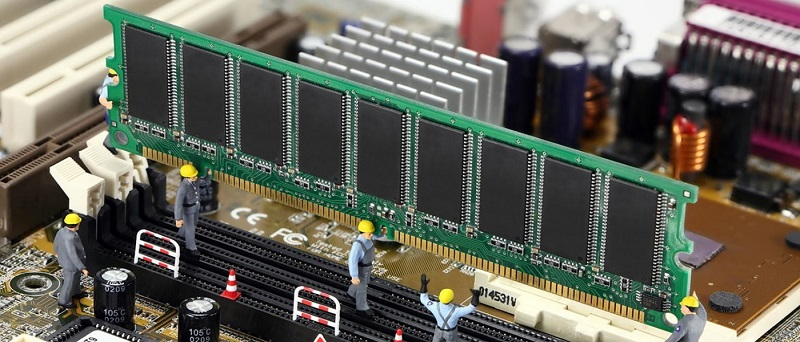
\includegraphics[width=0.75\textwidth]{ram.jpg}
    \caption{imagen ram}
    \label{fig:my_label}
\end{figure}
\subsection*{Memoria ROM(Memoria de solo lectura)}
Es el medio de almacenamiento de programas o datos que permiten el buen funcionamiento de los ordenadores o dispositivos electrónicos a través de la lectura de la información sin que pueda ser destruida o reprogramable.\\[0.1cm]
\begin{figure}[h]
    \centering
    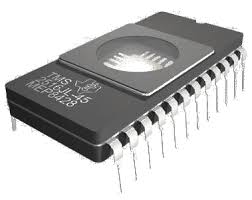
\includegraphics[width=0.75\textwidth]{rom.jpg}
    \caption{imagen ROM}
    \label{fig:my_label}
\end{figure}
\subsection*{Disco Duro}
Es un dispositivo de almacenamiento de datos que emplea un sistema de grabación magnética para almacenar y recuperar archivos digitales.
\begin{figure}[h]
    \centering
    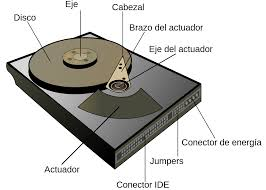
\includegraphics[width=0.75\textwidth]{disco.jpg}
    \caption{disco duro}
    \label{fig:my_label}
\end{figure}
\subsection*{3) Describa como se gestiona la memoria de un computador.}
De la gestion en el computador se encarga el procesador en cierta parte, aunque mayormente es gracias al administrador de memoria presente en los sistemas operativos y su labor consiste en llevar un registro de las partes de memoria que se estén utilizando y aquellas que no, con el fin de asignar espacio en memoria a los procesos cuando éstos la necesiten y liberándola cuando terminen. Así mismo sabe que información necesita ser cargada en RAM y cual no, y lo mismo para los otros tipos de memorias presentes como cache, vram, etc.
¿para qué sirve?
Para optimizar el espacio y poder cargar o intercambiar los programas que van a hacer ejecutados del disco duro a la memoria principal. Llevar un registro de las partes de la memoria que están en uso y de las que no. Si detecta que hay una parte que ya no está en uso, la libera para poder asignarla a los procesos que la necesiten. Facilitar un espacio de memoria para cada proceso y controlar que ninguno de ellos trabaje en zonas de memoria que no le han sido asignados. A el intercambio entre la memoria principal y el disco en los casos en los que la memoria principal no le pueda dar capacidad a todos los procesos que tienen necesidad de ella.\\[0.1cm]
\subsection*{4)¿Qué hace que una memoria sea más rápida que otra? ¿Por qué esto es importante?}
Lo que hace que una memoria sea más rápida que otra, radica en la forma en que se construye (funcionalidad), la velocidad de acceder a los datos, la capacidad, además de la velocidad de escritura y lectura. Esto permite crear memorias con un único propósito, a lo cual sería más eficiente (mas rápida), más fácil de crear en masa, de costo más bajo, mejor comunicación, entre otros muchos beneficios.










\end{document}
